\documentclass[conference]{IEEEtran}
\usepackage{graphicx}
\usepackage{booktabs}
\usepackage{amsmath}
\usepackage{url}
\usepackage[hidelinks]{hyperref}
\usepackage{cite}

\begin{document}

\title{Where Do Layout Detectors Fail on Indian Documents?\\ A Study of Script, Domain and Scan Quality on IndicDLP}

\author{
\IEEEauthorblockN{Prashant Jha, Aditya Soni, Riddhi Patil, Mariam Badure and Joanne Gomes}
\IEEEauthorblockA{Department of Artificial Intelligence and Machine Learning\\
St. Francis Institute of Technology (Autonomous), Mumbai, India}
}

\maketitle

\begin{abstract}
%%ABSTRACT%%
\end{abstract}

\begin{IEEEkeywords}
document layout analysis, Indian languages, object detection, robustness, cross-script generalisation, OCR
\end{IEEEkeywords}

%%STATIC%%

%%RESULTS%%

\section{The IndicDoc AI Tool}
We built a tool on the best detector of the study so that the results can be used, not only read. A user uploads
an image or a PDF page in a web app (Streamlit) or sends it to a REST API (FastAPI). The page goes through five
steps: (1) the released DocLayout-YOLO finds the regions; (2) boxes below the chosen confidence are dropped and
boxes that cover the same region with a different label are merged (IoU $>0.7$); (3) the region probe picks the
script; (4) Tesseract~5~\cite{tesseract} (\texttt{tessdata\_best}) reads the whole page once and each word is assigned to the region
that contains it, so that words outside every region are kept rather than lost; (5) regions are put in reading
order and returned as Markdown and JSON. The user can choose ``find every part'' (higher recall) or ``balanced''
(best F1); both thresholds were chosen on validation pages. Fig.~\ref{fig:app} shows a Tamil textbook page. The
tool runs in Docker without internet access; layout detection takes %%A_TIME%% s per page on an Apple M1 Pro GPU.

\begin{figure}[t]
\centering
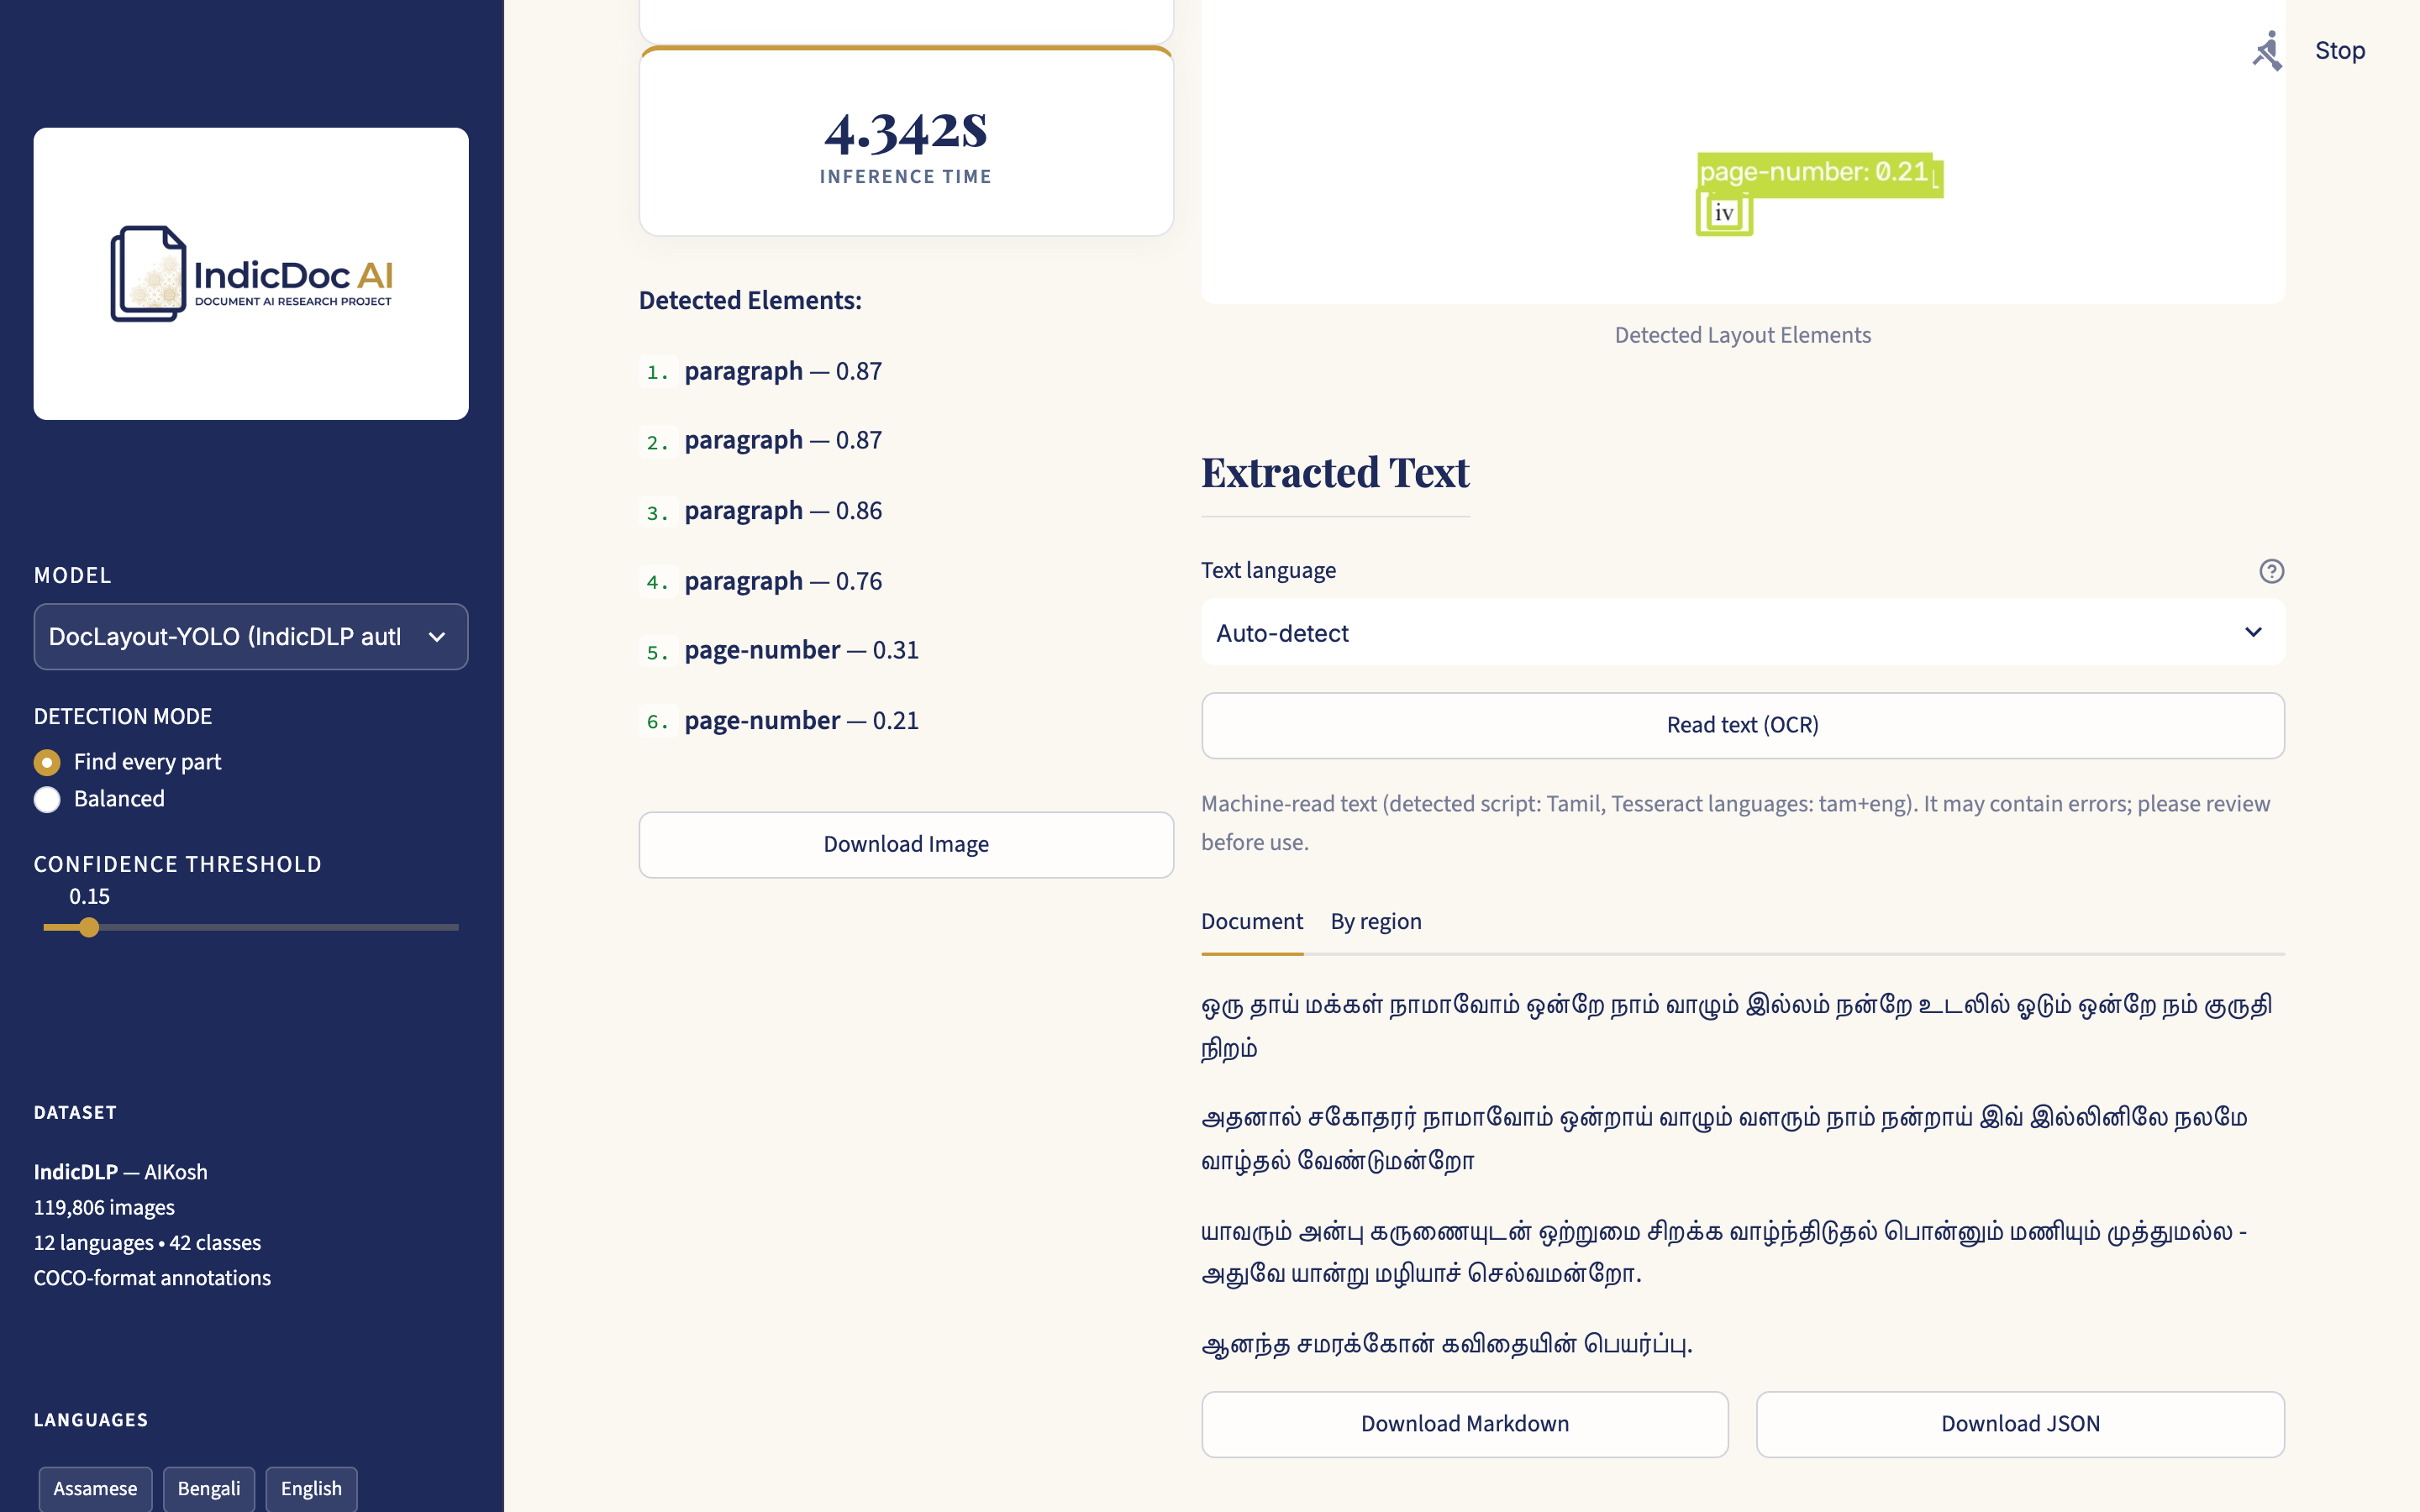
\includegraphics[width=\columnwidth]{figures/app_ocr.png}
\caption{IndicDoc AI on a Tamil textbook page: detected regions (left list) and the text read in reading order
with the script chosen automatically.}
\label{fig:app}
\end{figure}

\section{Discussion and Limitations}
\textbf{What the study suggests.} For someone who wants to process Indian documents, the choice of
\emph{document type} and \emph{scan quality} matters more than the language, once the script has been seen in
training. Forms, magazines and damaged pages are where effort should go: more labelled forms, and damage
augmentation during training. Simple ratios such as CI and RI make these weak spots visible in a way a
single mAP number does not.

\textbf{Limitations.} (1) We use a subset of %%TEST_PAGES%% test pages; Hindi has only 22 of them, so its
numbers are less certain. (2) Our own models were trained for about an hour on a laptop GPU with one random seed, and the robustness test covers the released model and our YOLOv8s only. (3) Scan damage was simulated;
real damage often combines several kinds at once. (4) IndicDLP has no text ground truth, so we could not measure
OCR character accuracy; we measured only script choice and how much text falls inside regions. (5) The released
detector was trained by the IndicDLP authors; we evaluate it but did not train it.

\section{Conclusion}
We studied where layout detectors fail on Indian-language documents instead of proposing a new detector. On
%%TEST_PAGES%% IndicDLP test pages, the released DocLayout-YOLO is accurate (%%A_MAP%% mAP@50) and fairly even across
the 12 languages, but much weaker on forms than on research papers, and it loses part of its accuracy on damaged
scans, most of all to blur. Choosing the OCR script by probing detected regions is far more reliable than
Tesseract's own detector. Future work: a controlled test of scripts never seen in training (same data size, with and without a script family), damage augmentation, more labelled forms, a stronger Indic OCR model with
a small text ground-truth set, and table structure and question answering on the detected tables. The code, the
data subset as CSV files and the tool are available to reviewers on request.

\section*{Acknowledgment}
We thank our guide Dr.~Joanne Gomes and the Department of AIML, SFIT. We thank the IndicDLP authors for releasing
their dataset and model.

\begin{thebibliography}{99}
\bibitem{indicdlp} O.~Nath, S.~Kukkala, M.~Khapra and R.~K.~Sarvadevabhatla, ``IndicDLP: A foundational dataset for multi-lingual and multi-domain document layout parsing,'' in \emph{Proc. ICDAR}, 2025, pp.~23--39.
\bibitem{doclayout} Z.~Zhao, H.~Kang, B.~Wang and C.~He, ``DocLayout-YOLO: Enhancing document layout analysis through diverse synthetic data and global-to-local adaptive perception,'' arXiv:2410.12628, 2024.
\bibitem{unitabbank} A.~Mondal \emph{et al.}, ``UniTabBank: A large scale multi-lingual, multi-layout, multi-type, multi-format dataset for table detection,'' in \emph{Proc. IEEE/CVF WACV}, 2026, pp.~6486--6495.
\bibitem{fasterrcnn} S.~Ren, K.~He, R.~Girshick and J.~Sun, ``Faster R-CNN: Towards real-time object detection with region proposal networks,'' in \emph{Proc. NeurIPS}, 2015.
\bibitem{yolov8} G.~Jocher, A.~Chaurasia and J.~Qiu, ``Ultralytics YOLOv8,'' 2023. [Online]. Available: \url{https://github.com/ultralytics/ultralytics}
\bibitem{platter} B.~V.~Kasuba, D.~Kudale, V.~Subramanian, P.~Chaudhuri and G.~Ramakrishnan, ``PLATTER: A page-level handwritten text recognition system for Indic scripts,'' arXiv:2502.06172, 2025.
\bibitem{hindiocr} S.~Bhattacharyya, S.~Ghosh, P.~Deb, A.~Mondal and C.~V.~Jawahar, ``Adapting vision-language models for Hindi OCR,'' IIIT Hyderabad, 2025.
\bibitem{layoutxlm} Y.~Xu \emph{et al.}, ``LayoutXLM: Multimodal pre-training for multilingual visually-rich document understanding,'' arXiv:2104.08836, 2021.
\bibitem{drishtikon} B.~V.~Kasuba, P.~Chaudhuri and G.~Ramakrishnan, ``DRISHTIKON: Visual grounding at multiple granularities in documents,'' arXiv:2506.21316, 2025.
\bibitem{tableqa} V.~Pal, E.~Kanoulas, A.~Yates and M.~de~Rijke, ``Table question answering for low-resourced Indic languages,'' arXiv:2410.03576, 2024.
\bibitem{devtables} A.~R.~Dumada and S.~G.~Shah, ``Incorporate structure and content for Devanagari table extraction,'' \emph{IJSAT}, vol.~17, no.~1, 2026.
\bibitem{hendrycks} D.~Hendrycks and T.~Dietterich, ``Benchmarking neural network robustness to common corruptions and perturbations,'' in \emph{Proc. ICLR}, 2019.
\bibitem{coco} T.-Y.~Lin \emph{et al.}, ``Microsoft COCO: Common objects in context,'' in \emph{Proc. ECCV}, 2014.
\bibitem{tesseract} R.~Smith, ``An overview of the Tesseract OCR engine,'' in \emph{Proc. ICDAR}, 2007.
\end{thebibliography}

\end{document}
